\chapter{Theory}
\label{chap:theory}
In this section, the theoretical modelling of the bicycle and the data driven Min-Max MPC is discussed.

Since the objective of this research is to simply balance the bicycle, a simple kinetic model is sufficient for this purpose. We use two models and compare between them in terms of control and balance.
The difference between both models is considering the fork angle.
The fork axis inclination introduces the castor effect which is studied in \cite{yu2018}.
For controlling the bicycle, the data-driven MPC is compared with an LQR contoller and is applied in simulation and on a real model-scale bicycle to assess the controllers. In this chapter, the bicycle model used is discussed and the theory behind the data-driven state-feedback controller is explained.

\section{Bicycle Modelling}
\label{sec:bike_modelling}
	To model the riderless bicycle, it can be treated as an inverted pendulum. There are some (assumptions) parameters that are neglected such as: elasticity of bicycle parts, the tire-road friction, etc. A simple second-order model of the bicycle can be derived given that the rear-speed is constant, the bicycle rolling on the horizontal plane, and initially, the steer axis $\lambda$ is in a vertical position as in Figure \ref{fig:bike_model}. Using the Conservation of Angular Momentum, the following Equation \ref{eq:bike_second_order} is acquired to balance the bicycle.
	\begin{equation}
		\label{eq:bike_second_order}
		\ddot{\varphi} - \frac{g}{h} \varphi = - \frac{av}{hl} \dot{\delta} - \frac{v^2}{h l} \delta,
	\end{equation}

	where $\varphi$ is the lean angle, $\delta$ is the steer angle, $g$ is the gravity acceleration, $h$ is the height of the center of mass, $l$ is the wheelbase, $a$ is the distance from the center of mass to the front wheel and $v$ is the speed of the bicycle. The bicycle model is a second-order system with two states: lean angle $\varphi$ and steer angle $\delta$.
	This is based on linearisation where the desired stability steady-state for both angles $\delta$ and $\phi$ is 0.

	Now, to consider the fork angle $\lambda$, which is shown in \autoref{fig:fork_model}, Equation \eqref{eq:bike_second_order} is expanded as follows.
		\begin{equation}
		\label{eq:bike_second_order_fork}
		\ddot{\varphi} - \frac{g}{h} \varphi = - \frac{av \sin \lambda}{hl} \dot{\delta} - \frac{\left(v^2 h - ar_\tau g \right) \sin \lambda}{h^2 l} \delta,
	\end{equation}
		where $\lambda$ is the fork angle, and $r_\tau$ is the trail distance such that $r_\tau = \tan(\frac{\pi}{2} - \lambda) $.
	It is clear that the difference between both \eqref{eq:bike_second_order} and \eqref{eq:bike_second_order_fork} is putting the fork angle $\lambda = 90\degree$ and $r_{\tau} = 0$.
	The state-space representation of the system model considering the fork angle given by Equation \ref{eq:bike_second_order_fork} is
	\begin{equation}
		\label{eq:bike_state_equation}
		\begin{bmatrix}
			\dot{\varphi} \\
			\ddot{\varphi} \\
			\dot{\delta}
		\end{bmatrix}
		=
		\begin{bmatrix}
			0 & 1 & 0 \\
			\frac{g}{h} & 0 & \frac{\left(a r_\tau g - v^2 h \right) \sin \lambda}{h^2 l} \\
			0 & 0 & 0
		\end{bmatrix}
		\begin{bmatrix}
			\varphi \\
			\dot{\varphi} \\
			\delta
		\end{bmatrix}
		+
		\begin{bmatrix}
			0 \\
			\frac{- a v \sin \lambda}{h l} \\
			1
		\end{bmatrix}
		\dot{\delta}.
	\end{equation}

%\begin{figure}[htbp]
%	\centering
%	\begin{subfigure}[b]{0.78\textwidth}
%		\centering
%		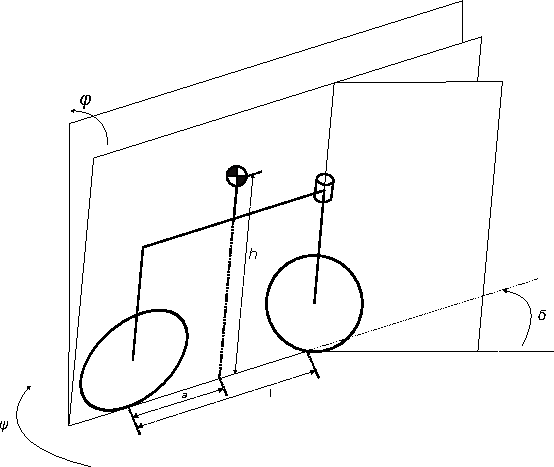
\includegraphics[width=\linewidth]{figures/minibike/model.pdf}
%		\caption{Kinematic no-fork model of the bicycle.}
%		\label{fig:bike_model}
%	\end{subfigure}
%	\hfill
%	\begin{subfigure}[b]{0.20\textwidth}
%		\centering
%		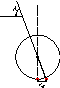
\includegraphics[width=\linewidth]{figures/minibike/fork_angle_half_final.pdf}
%%		\caption{Fork model showing the steering axis inclined by angle \( \lambda \), introducing a trail distance \( r_{\tau} \).}
%		\label{fig:fork_model}
%	\end{subfigure}
%	\caption{Illustration of bicycle models used in the analysis. (a) shows the simplified kinematic model without a front fork. (b) highlights the fork geometry with a non-zero head angle \( \lambda \) and trail \( r_{\tau} \), affecting steering dynamics.}
%	\label{fig:bike_models_combined}
%\end{figure}
\begin{figure}[H]
	\centering
	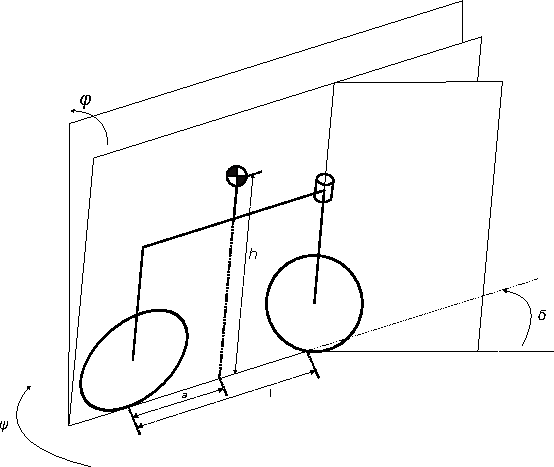
\includegraphics[width=\linewidth]{figures/minibike/model.pdf}
	\caption{A Kinetic no-fork model of the bicycle }
	\label{fig:bike_model}
\end{figure}
\begin{figure}[H]
	\centering
	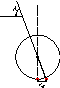
\includegraphics[width=0.25\linewidth]{figures/minibike/fork_angle_half_final.pdf}
	\caption{A fork model showing an inclination with angle $\lambda$ of the steering axis, introducing a trail distance $r_{tau}$.}
	\label{fig:fork_model}
\end{figure}
\section{Data-Driven Min-Max MPC}
\label{sec:data_driven_mpc}
In this section, we show how to derive the Data-Driven Min-Max MPC mentioned in \cite{xie2024}.
To formulate our problem, we consider a discrete-time \gls{lti} system affected by process noise:
	\begin{equation}
		\label{eq:system}
		x_{t+1} = A_s x_t + B_s u_t + \omega_t,
	\end{equation}
where \(x_t, x_{t+1} \in \mathbb{R}^n\) are the state vectors, \(u_t \in \mathbb{R}^m\) is the control input, and \(\omega_t \in \mathbb{R}^n\) represents unknown but bounded disturbance at time \(t\).
The system matrices \(A_s\) and \(B_s\) are assumed to be unknown.
Instead of identifying a model explicitly, we utilize available noisy input-state data to design a stabilizing controller.
The noise \(\omega_t\) is assumed to satisfy a known upper bound $\epsilon \geq 0$ such that
\[
\|\omega_t\|_2^2 \leq \varepsilon.
\]

To move to the data-driven framework, a data sequence consisting of states $x_i$, inputs $u_i$, and process noise $\omega_i$ where $i \in \mathbb{N}$ is considered. The system in \autoref{eq:system} can then be rewritten in terms of the data sequence as
    \begin{equation} \label{eq:system_omega}
		\omega_i = x_{i+1} - A_s x_i - B_s u_i,
	\end{equation}
where $i \in \mathbb{N}$ denotes the data index.
Let the pair \(\left(A, B\right)\) be the set of system matrices that satisfy \autoref{eq:system_omega} and the noise bound. This set of system matrices can be written as the following quadratic matrix inequality
	\begin{equation}
		\Sigma_i = \left\{ \left( A, B \right) :
		\begin{bmatrix} I & A & B \end{bmatrix}
		\begin{bmatrix}
			I & x_{i+1} \\
			0 & -x_i \\
			0 & -u_i
		\end{bmatrix}
		\begin{bmatrix}
			\epsilon I & 0 \\
			0 & -I
		\end{bmatrix}
		\begin{bmatrix}
			I & 0 & 0 \\
			x_{i+1} & -x_i & -u_i
		\end{bmatrix}
		\begin{bmatrix} I \\ A \\ B \end{bmatrix}
		\succeq 0
		\right\}.
\end{equation}
Then, the set of system matrices consistent with all data points can be described as follows
	\begin{equation}
		\mathcal{C} = \bigcap_{i=0}^{T-1} \Sigma_i,
	\end{equation}
\noindent
which is equivalent to the following quadratic matrix inequality
	\begin{equation}
		\mathcal{C} = \left\{ \left( A, B \right) :
		\begin{bmatrix} I & A & B \end{bmatrix}
		\Pi(\tau)
		\begin{bmatrix} I & A & B \end{bmatrix}^\top \succeq 0,\,
		\forall \tau = \left(\tau_0, \ldots, \tau_{T-1}\right),\, \tau_i \geq 0,\, i \in \mathbb{I}_{[0,T-1]}
		\right\},
	\end{equation}
where $\Pi(\tau)$ is
\begin{equation}
	\label{eq:PI}
	\Pi(\tau) = \sum_{i=0}^{T-1} \tau_i
	\begin{bmatrix}
		I & x_{i+1} \\
		0 & -x_i \\
		0 & -u_i
	\end{bmatrix}
	\begin{bmatrix}
		\epsilon I & 0 \\
		0 & -I
	\end{bmatrix}
	\begin{bmatrix}
		I & x_{i+1} \\
		0 & -x_i \\
		0 & -u_i
	\end{bmatrix}^{\top}.
\end{equation}

To design a control law that stabilises the system despite the uncertainty in \((A, B)\), we setup the problem by defining a quadratic stage cost function as
\[
%l(u, x) = \|u\|_R^2 + \|x\|_Q^2,
l(u, x) = u^\top R u + x^\top Q x,
\]
where \(\ell(x, u) = x^\top Q x + u^\top R u\) is the quadratic stage cost, with weighting matrices \(Q \succ 0\) and \(R \succ 0\).
such that the weighting matrices $R, Q \succ 0$.
In addition, we define state and input ellipsoidal constraints by the following
\[
\|u_t\|_{S_u} \leq 1, \quad \|x_t\|_{S_x} \leq 1, \quad \forall t \in \mathbb{N},
\]
where $S_u \succ 0$, $S_x \succeq 0$, and $\|x\|_P = \sqrt{x^\top P x}$.
Now, we can state a data-driven min-max MPC problem at time $t$ by
%\[
%\min_{u(\cdot)} \max_{(A, B) \in \mathcal{C}} \sum_{k=0}^{\infty} \ell(x_k, u_k),
%\]

\begin{subequations} \label{eq:main_problem}
	\begin{align}
		J_\infty^*(x_t) &:= \min_{\bar{u}(t)} \max_{(A, B) \in \mathcal{C}} \sum_{k=0}^{\infty} l\left(\bar{u}_k(t), \bar{x}_k(t)\right) \\
		\text{s.t.} \quad & \bar{x}_{k+1}(t) = A \bar{x}_k(t) + B \bar{u}_k(t), \label{subeq:b}\\
		& \bar{x}_0(t) = x_t, \label{subeq:c}\\
		& \|\bar{u}_k(t)\|_{S_u} \leq 1, \ \forall t \in \mathbb{N}, \label{subeq:d}\\
		& \|\bar{x}_k(t)\|_{S_x} \leq 1, \ \forall \left(A, B\right) \in \mathcal{C}, \ t \in \mathbb{N} \label{subeq:e}.
	\end{align}
\end{subequations}
%
This cost function can be explained by being a minimisation of the worst-case cost $l$ over all system matrices in $\mathcal{C}$ by adjusting the input $\bar{u}_k(t), \forall k \in \mathbb{N}$ to the system. $\bar{x}_k(t)$ is the predicted state and $\bar{u}_k(t)$ is the control input, both at time step $t+k$.
The sets $(A,B)$ used are consistent with the system dynamics in \eqref{subeq:b}. We let the initial state be the measurement state $x_t$ as shown in constraint \eqref{subeq:c}.
The ellipsoidal constraints for the control input and states are given in constraints \eqref{subeq:d} and \eqref{subeq:e} respectively.

Now, the data-driven min-max MPC can be simplified by just considering a state-feedback control law, such that $u_t = F_t x_t$, where $F_t \in R^{m \times n}$.

In \cite{xie2024}, it is shown that the data-driven min-max MPC in \autoref{eq:main_problem} can be reformulated as an SDP.
Suppose that there exist $\gamma > 0$, $H \in \mathbb{R}^{n \times n}$, $L \in \mathbb{R}^{m \times n}$, $\tau \in \mathbb{R}^T$.
The SDP problem is expressed as the following
\begin{subequations} \label{eq:final_gamma}
	\begin{gather}
		\minimise_{\gamma, H, L, \tau} \gamma \\
		\text{s.t.} \nonumber \text{the following LMIs hold} \nonumber
		\\
		\begin{bmatrix} \label{subeq:LMI_b_constraints}
			1 & x_t^\top \\
			x_t & H
		\end{bmatrix} \succeq 0,
		\\
		\begin{bmatrix} \label{subeq:LMI_c_constraints}
			\begin{bmatrix}
				-H & 0 \\
				0 & 0
			\end{bmatrix}
			+
			\Pi(\tau)
			&
			\begin{bmatrix}
				0 \\
				H \\
				L
			\end{bmatrix}
			&
			0 \\
			\begin{bmatrix}
				0 & H & L^\top
			\end{bmatrix}
			& -H & \Phi^\top \\
			0 & \Phi & -\gamma I
		\end{bmatrix} \prec 0,
		\\
		\tau = (\tau_0, \ldots, \tau_{T-1}), \ \tau_i \geq 0, \ \forall i \in \mathbb{I}_{[0, T-1]}, \label{subeq:LMI_d_constraints}
		\\
		\begin{bmatrix}
			H & L^\top \\
			L & S_u^{-1}
		\end{bmatrix} \succeq 0, \label{subeq:LMI_e_constraints}
		\\
		\begin{bmatrix} \label{subeq:LMI_f_constraints}
			S_x & I \\
			I & H
		\end{bmatrix} \succeq 0.
	\end{gather}
\end{subequations}
where $\Phi = \begin{bmatrix} M_R L \\ M_Q H \end{bmatrix}$ and $M_R^\top M_R = R$, $M_Q^\top M_Q = Q$.
The $\gamma$ upper bounds the optimal cost in \autoref{eq:main_problem}.
The LMIs \eqref{subeq:LMI_b_constraints}, \eqref{subeq:LMI_c_constraints}, and \eqref{subeq:LMI_d_constraints} ensure that the system dynamics with the bounded noise are satisfied. While the LMIs \eqref{subeq:LMI_e_constraints} and \eqref{subeq:LMI_f_constraints} define the state and input constraints.
The optimal solution for the problem \eqref{eq:final_gamma} is then expressed as $\gamma^\star, \, H^\star, \, L^\star, \, \tau^\star$. Consequently, the optimal state-feedback gain is $F = L^\star (H^\star)^{-1}$.

The SDP problem is then solved in a receding horizon manner as per Algorithm \autoref{alg:algorithm_MPC}. At a time-step $t$, \eqref{eq:final_gamma} is solved and the state-feedback gain $F_t$ is acquired and then the first input $u_t = F_t x_t$ is applied.

\begin{algorithm}
	\caption{Data-driven min-max MPC}
%	\label{alg:algorithm_MPC}
	\begin{algorithmic}[1]
		\STATE At time $t = 0$, measure state $x_0$;
		\STATE Solve the problem \eqref{eq:final_gamma};
		\STATE Apply the input $u_t = F_t x_t$;
		\STATE Set $t = t + 1$ and go back to 2;
	\end{algorithmic}
	\label{alg:algorithm_MPC}
\end{algorithm}

%The optimal feedback gain \(K\) is obtained by solving a convex semidefinite program (SDP) derived from the min-max formulation.
%Specifically, there exists a positive definite matrix \(P\) such that for all \((A, B) \in \mathcal{C}\), the following holds:
%\[
%(A + B K)^\top P (A + B K) - P + Q + K^\top R K \preceq 0.
%\]
%This inequality ensures that the closed-loop system is exponentially stable and satisfies the cost decrease condition.
%
%The SDP formulation allows the computation of \(K\) directly from the noisy input-state data without requiring explicit model identification.


%
%\begin{framed}
%	\noindent
%	\textbf{Main Optimization Problem: Data-Driven Min-Max MPC}
%
%	\vspace{0.3em}
%	Given collected input-state data, the data-driven min-max control problem seeks a state-feedback gain \(F_t\) minimizing the worst-case infinite-horizon cost:
%	\[
%	\min_{\bar{u}(t)} \max_{(A, B) \in \mathcal{C}} \sum_{k=0}^{\infty} x_k^\top Q x_k + \bar{u}_k^\top R u_k
%	\]
%	given an initial state $x_t$ subject to some input and state constraints and the corresponding consistent set of system matrices \(\mathcal{C}\).
%
%	The SDP reformulation of the optimisation problem is as follows:
%	\begin{subequations}\nonumber %\label{eq:final_gamma}
%		\begin{gather}
%			\minimise_{\gamma, H, L, \tau} \gamma \\
%			\text{s.t. the following LMIs}
%		\end{gather}
%	\end{subequations}
%	\begin{subequations}\nonumber %\label{SDP_LMIs}
%		\begin{gather}
%			\begin{bmatrix}
%				1 & x_t^\top \\
%				x_t & H
%			\end{bmatrix} \succeq 0,
%			\\
%			\begin{bmatrix}
%				\begin{bmatrix}
%					-H & 0 \\
%					0 & 0
%				\end{bmatrix}
%				+
%				\Pi(\tau)
%				&
%				\begin{bmatrix}
%					0 \\
%					H \\
%					L
%				\end{bmatrix}
%				&
%				0 \\
%				\begin{bmatrix}
%					0 & H & L^\top
%				\end{bmatrix}
%				& -H & \Phi^\top \\
%				0 & \Phi & -\gamma I
%			\end{bmatrix} \prec 0,
%			\\
%			\tau = (\tau_0, \ldots, \tau_{T-1}), \ \tau_i \geq 0, \ \forall i \in \mathbb{I}_{[0, T-1]},
%		\end{gather}
%	\end{subequations}
%	\begin{subequations} \nonumber
%		\begin{gather}
%			\begin{bmatrix}
%				H & L^\top \\
%				L & S_u^{-1}
%			\end{bmatrix} \succeq 0,
%			\\
%			%		\quad
%			\begin{bmatrix}
%				S_x & I \\
%				I & H
%			\end{bmatrix} \succeq 0.
%		\end{gather}
%	\end{subequations}
%%	subject to the closed-loop dynamics:
%%	\[
%%	x_{k+1} = (A + B K) x_k
%%	\]
%%	and input-state constraints (if any).
%
%%	This is reformulated as a semidefinite program (SDP) that searches for a positive definite matrix \(P \succ 0\) and feedback gain \(K\) satisfying:
%%	\[
%%	(A + B K)^\top P (A + B K) - P + Q + K^\top R K \preceq 0, \quad \forall (A, B) \in \mathcal{C}.
%%	\]
%
%	\vspace{0.5em}
%%	The resulting controller guarantees robust exponential stability and constraint satisfaction for all systems compatible with the observed data.
%\end{framed}
